\subsection{RQ1: To what extent can different language models generate correct code?}

\newcommand{\score}[1]{%
  \ifdim #1pt < 25pt \cellcolor{red!20}#1%
  \else\ifdim #1pt < 50pt \cellcolor{orange!20}#1%
  \else\ifdim #1pt < 75pt \cellcolor{yellow!30}#1%
  \else\cellcolor{green!30}#1%
  \fi\fi\fi%
}

\newcommand{\scorecell}[2]{%
  \ifdim #1pt < 25pt \cellcolor{red!20}#2%
  \else\ifdim #1pt < 50pt \cellcolor{orange!20}#2%
  \else\ifdim #1pt < 75pt \cellcolor{yellow!30}#2%
  \else\cellcolor{green!30}#2%
  \fi\fi\fi%
}

\begin{figure}[htbp]
\centering
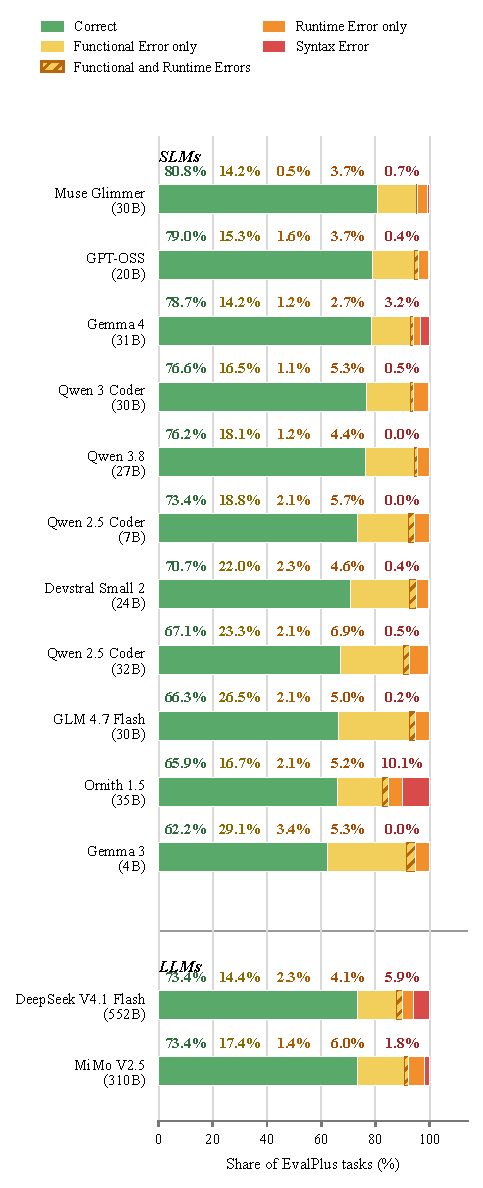
\includegraphics[width=\columnwidth]{figures/code_generation_results.pdf}
\caption{Code-generation outcomes across the 563 EvalPlus tasks. Each horizontal bar partitions the tasks into mutually exclusive outcomes; diagonal hatching marks programs labeled with both Functional and Runtime Errors. The five values above each bar report, respectively, Correct, Functional Error only, Functional and Runtime Errors, Runtime Error only, and Syntax Error.}
\label{fig:rq1_generation}
\end{figure}

Figure ~\ref{fig:rq1_generation} shows that, across all evaluated models, correct classification is the most common result, even though accuracy varies across configurations. This variation is most evident in the most notable results, such as Muse Glimmer 30B, with an accuracy of 80.8\%, and Gemma 3 4B, which had the lowest accuracy at 62.2\%. These results show that the SLMs can produce correct results and that different configurations yield significant differences.

Although model size is a determining factor in these differences, it is not the only one that guarantees superior performance. For example, in the Qwen 2.5 model family, the 7B configuration showed a hit rate of 73.8\%, while the 32B achieved 67.1\%. This demonstrates that larger models do not always outperform smaller ones in this protocol. However, this observation cannot be generalized, since the best results come from larger models, such as Muse Glimmer 30B and Gemma 4 31B.

The error distribution shows how code generation fails. Specifically, errors classified as functional are the most common, representing 15 to 30\% of generations, while runtime errors are less common, at 4 to 9\%. Therefore, the main difficulty lies in producing code that fully meets task requirements, rather than code that doesn't fail during execution.

\begin{table*}[htbp]
\centering
\caption{Error-detection performance by model (\%). CR, FR, RR, and SR denote recall for Correct, Functional Error, Runtime Error, and Syntax Error, respectively. MF1(NS) denotes Macro-F1 computed without the Syntax Error class.}
\label{tab:rq2_detection}
\begin{tabular}{lrrrrrrr}
\toprule
\textbf{Model} &
\textbf{Acc} &
\textbf{MF1} &
\textbf{CR} &
\textbf{FR} &
\textbf{RR} &
\textbf{SR} &
\textbf{MF1(NS)} \\
\midrule

\multicolumn{8}{l}{\emph{General-purpose models}} \\
\midrule

Muse Glimmer 30B
& \score{73.1}
& \score{53.8}
& \score{83.3}
& \score{55.5}
& \score{27.0}
& \score{52.9}
& \scorecell{61.3}{61.3 (+7.5)}
\\

Gemma 4 31B
& \score{72.4}
& \score{48.5}
& \score{83.7}
& \score{50.1}
& \score{24.1}
& \score{78.4}
& \scorecell{55.8}{55.8 (+7.3)}
\\

Qwen 3.8 27B
& \score{62.6}
& \score{42.6}
& \score{62.9}
& \score{75.9}
& \score{12.7}
& \score{64.7}
& \scorecell{48.6}{48.6 (+5.9)}
\\

Qwen 2.5 Coder 7B
& \score{62.5}
& \score{33.7}
& \score{72.3}
& \score{46.7}
& \score{2.5}
& \score{17.6}
& \scorecell{39.4}{39.4 (+5.7)}
\\

Qwen 2.5 Coder 32B
& \score{60.8}
& \score{41.0}
& \score{71.1}
& \score{38.1}
& \score{11.4}
& \score{76.5}
& \scorecell{43.3}{43.3 (+2.3)}
\\

Qwen 3 Coder 30B
& \score{60.6}
& \score{37.8}
& \score{63.8}
& \score{65.9}
& \score{9.3}
& \score{21.6}
& \scorecell{44.1}{44.1 (+6.3)}
\\

Ornith 1.5 35B
& \score{56.3}
& \score{35.7}
& \score{55.4}
& \score{78.1}
& \score{8.0}
& \score{35.3}
& \scorecell{43.1}{43.1 (+7.4)}
\\

Devstral Small 2 24B
& \score{53.9}
& \score{38.1}
& \score{54.9}
& \score{63.6}
& \score{17.7}
& \score{35.3}
& \scorecell{43.3}{43.3 (+5.2)}
\\

GLM 4.7 Flash 30B
& \score{50.4}
& \score{37.3}
& \score{49.3}
& \score{64.0}
& \score{26.2}
& \score{94.1}
& \scorecell{43.5}{43.5 (+6.3)}
\\

Gemma 4 E2B IT
& \score{48.1}
& \score{33.1}
& \score{47.8}
& \score{65.4}
& \score{16.5}
& \score{5.9}
& \scorecell{40.6}{40.6 (+7.5)}
\\

Gemma 4 E4B IT
& \score{45.9}
& \score{37.0}
& \score{38.0}
& \score{86.4}
& \score{31.6}
& \score{47.1}
& \scorecell{41.8}{41.8 (+4.7)}
\\

Gemma 3 4B IT
& \score{38.5}
& \score{26.7}
& \score{30.0}
& \score{82.0}
& \score{10.1}
& \score{5.9}
& \scorecell{32.4}{32.4 (+5.7)}
\\

Gemma 3 4B
& \score{32.9}
& \score{23.4}
& \score{22.6}
& \score{84.7}
& \score{6.3}
& \score{17.6}
& \scorecell{27.3}{27.3 (+3.9)}
\\

GPT-OSS 20B
& \score{25.1}
& \score{39.0}
& \score{17.5}
& \score{55.8}
& \score{32.9}
& \score{72.5}
& \scorecell{40.4}{40.4 (+1.4)}
\\

\midrule
\multicolumn{8}{l}{\emph{Fine-tuned models}} \\
\midrule

Best Acc
& \score{77.8}
& \score{50.9}
& \score{85.3}
& \score{69.1}
& \score{27.8}
& \score{11.8}
& \scorecell{63.1}{63.1 (+12.2)}
\\

Weighted MF1
& \score{73.5}
& \score{54.2}
& \score{75.9}
& \score{77.9}
& \score{32.9}
& \score{64.7}
& \scorecell{62.9}{62.9 (+8.7)}
\\

Balanced Acc
& \score{67.8}
& \score{38.1}
& \score{74.4}
& \score{65.8}
& \score{15.2}
& \score{0.0}
& \scorecell{50.9}{50.9 (+12.7)}
\\

Balanced MF1
& \score{63.7}
& \score{36.0}
& \score{68.6}
& \score{65.8}
& \score{13.9}
& \score{0.0}
& \scorecell{48.0}{48.0 (+12.0)}
\\

\midrule
\multicolumn{8}{l}{\emph{Large models}} \\
\midrule

DeepSeek V4.1 Flash
& \score{75.5}
& \score{51.0}
& \score{89.3}
& \score{51.6}
& \score{14.8}
& \score{35.3}
& \scorecell{54.1}{54.1 (+3.1)}
\\

MiMo V2.5
& \score{51.5}
& \score{39.7}
& \score{47.2}
& \score{79.7}
& \score{21.5}
& \score{96.1}
& \scorecell{44.7}{44.7 (+5.0)}
\\

\bottomrule
\end{tabular}
\end{table*}


Syntax error classification is rare in most models, occurring in at most 3\%; however, some configurations show error patterns. The most notable case is Ornith 1.5 35B, which classifies about 10\% of generations as syntax errors, 91.2\% of which result from violations of the expected output structure. Furthermore, in most other models, only 20\% of syntax errors are Python grammar errors. Thus, syntax errors are not limited to grammar; instead, they occur predominantly in specific patterns, according to the parameters used in the study.

In summary, the evaluated models generally produce Python code with executable structures, but the main concern is behavior that diverges from expectations, even in the most robust models that achieve accuracy close to four-fifths. Furthermore, although less frequent, syntax errors follow patterns that depend on the model used. Additionally, analysis of the Qwen 2.5 family shows that accuracy rates depend not only on model size, although it is an important factor, but primarily on configuration.